
%\documentclass[10pt,a4paper]{article}
\documentclass[runningheads]{llncs}
\usepackage[utf8]{inputenc}
\usepackage{amsmath}
\usepackage{amsfonts}
\usepackage{amssymb}


\usepackage{thmtools}
%\usepackage{amsthm}
\usepackage{thm-restate}
%\declaretheorem[name=Theorem,numberwithin=section]{thm}
%--experiment

\usepackage%[hidelinks]
			{hyperref}

\usepackage[capitalize, noabbrev]{cleveref}
\usepackage[autostyle=true]{csquotes}
\usepackage{graphicx}
\usepackage{color}
\usepackage{enumerate}
\usepackage{caption}
\usepackage{subcaption}


% Abstand obere Blattkante zur Kopfzeile ist 2.54cm - 15mm
%\setlength{\topmargin}{-15mm}


% Umgebungen für Definitionen, Sätze, usw.
% Es werden Sätze, Definitionen etc innerhalb einer Section mit
% 1.1, 1.2 etc durchnummeriert, ebenso die Gleichungen mit (1.1), (1.2) ..
%\newtheorem{theorem}{Theorem}[section]
%\newtheorem{definition}[theorem]{Definition} 
%\newtheorem{lemma}[theorem]{Lemma}
%\newtheorem{corollary}[theorem]{Corollary}	
%\newtheorem{example}[theorem]{Example}
%\newtheorem{observation}[theorem]{Observation}	
%\newtheorem{conjecture}[theorem]{Conjecture}
%\newtheorem{question}[theorem]{Question}			   
                  
\numberwithin{equation}{section}

\newcommand{\R}{\mathbb{R}}
\newcommand{\N}{\mathbb{N}}
\newcommand{\Z}{\mathbb{Z}}
\newcommand{\set}[1]{\{ #1 \}}
\newcommand{\fromto}[2]{\set{#1, \ldots, #2}}

\newcommand{\comment}[1]{\textcolor{red}{(L: #1)}}

\newcommand{\bigO}{\mathcal{O}}
\newcommand{\dotunion}{\mathbin{\dot{\cup}}}

\newcommand{\act}{\textsc{(Act)}}
\newcommand{\stact}{\textsc{(stAct)}}
\newcommand{\activation}{\textsc{Activation}}
\newcommand{\stactivation}{\textsc{st-Activation}}
\newcommand{\True}{\textsc{True}}
\newcommand{\False}{\textsc{False}}

\DeclareMathOperator{\ac}{\text{A}}
\DeclareMathOperator{\val}{\text{value}}
\newcommand{\vall}{w}
\DeclareMathOperator{\radius}{\text{radius}}

\DeclareMathOperator{\Nout}{N^\text{out}}
\DeclareMathOperator{\Nin}{N^\text{in}}
\DeclareMathOperator{\dom}{dom}
\DeclareMathOperator{\tw}{tw}
\DeclareMathOperator{\transhull}{trans-hull}
\DeclareMathOperator{\opt}{OPT}
\newcommand{\optAct}{\opt_\text{ACT}}
\newcommand{\optStAct}{\opt_\text{stACT}}
\newcommand{\optMenger}{\opt_\text{MENGER}}
\newcommand{\optSTP}{\opt_\text{STP}}
\newcommand{\optDirStAct}{\opt_\text{STACT}}
\newcommand{\optDirMenger}{\opt_\text{dir-MENGER}}
\newcommand{\optDirAct}{\opt_\text{dir-ACT}}
\newcommand{\optDirSTP}{\opt_\text{dir-STP}}


\begin{document}

\title{$s$-$t$-Activation Draft}
%
%\titlerunning{Abbreviated paper title}
% If the paper title is too long for the running head, you can set
% an abbreviated paper title here
%
\author{Stefan Lendl\inst{1} \and
Gerhard Woeginger\inst{2} \and
Lasse Wulf\inst{3}}
%
\authorrunning{S. Lendl, G. Woeginger, L. Wulf}
% First names are abbreviated in the running head.
% If there are more than two authors, 'et al.' is used.
%
\institute{
Department of Operations and Information Systems, University of Graz, Austria 
\email{stefan.lendl@uni-graz.at}\\
\and Department of Algorithmics and Complexity, RWTH Aachen, Germany 
\email{woeginger@algo.rwth-aachen.de}\\
\and Institute of Discrete Mathematics, Graz University of Technology, Austria\\
\email{wulf@math.tugraz.at}
}
%
\maketitle              % typeset the header of the contribution
%
\section{Hardness}
\subsection{$s$-$t$-Activation Problem}
We now show hardness of the problem $\stact$, even if either the structure or the weights of the input are restricted. We begin with the case of restricted structure.

\begin{theorem}
\label{thm_stact_np_hard}
The problem \stact\ is NP-complete, even if the input graph is planar with treewidth at most 3.
\end{theorem}

\begin{proof}
Let $A = \fromto{a_1}{a_n}$ be an instance of \textsc{Partition} and $Q := 1/2 \sum A$. Consider the digraph from \cref{fig_stact_np_hard}. (By the symbol $\infty$, we mean a weight large enough, such that the corresponding edge is w.l.o.g.\ always active. For example, $\infty \geq 4Q$ suffices.) We claim that there exists a schedule of value $4Q$ if and only if $A$ is a yes-instance. Suppose $\sigma$ is such a schedule. By symmetry we can assume $\sigma((s,v_1)) = \sigma((v_1, z_1)) = 0$. Then also $\sigma((v_1, z
_2)) = Q$, otherwise we are inefficient and $\sigma$ can not have a value of $4Q$ (consider the cut $\delta(s)$). Then by a similar reasoning concerning efficiency, the scheduling of the edges between $z_1$ and $t$ implies a partition of $A$ into two equal parts. The other direction of the claim is easy to see. Finally, note that the involved graph is 
planar and has treewidth 3.
\end{proof}
\begin{figure}[htpb]
\centering
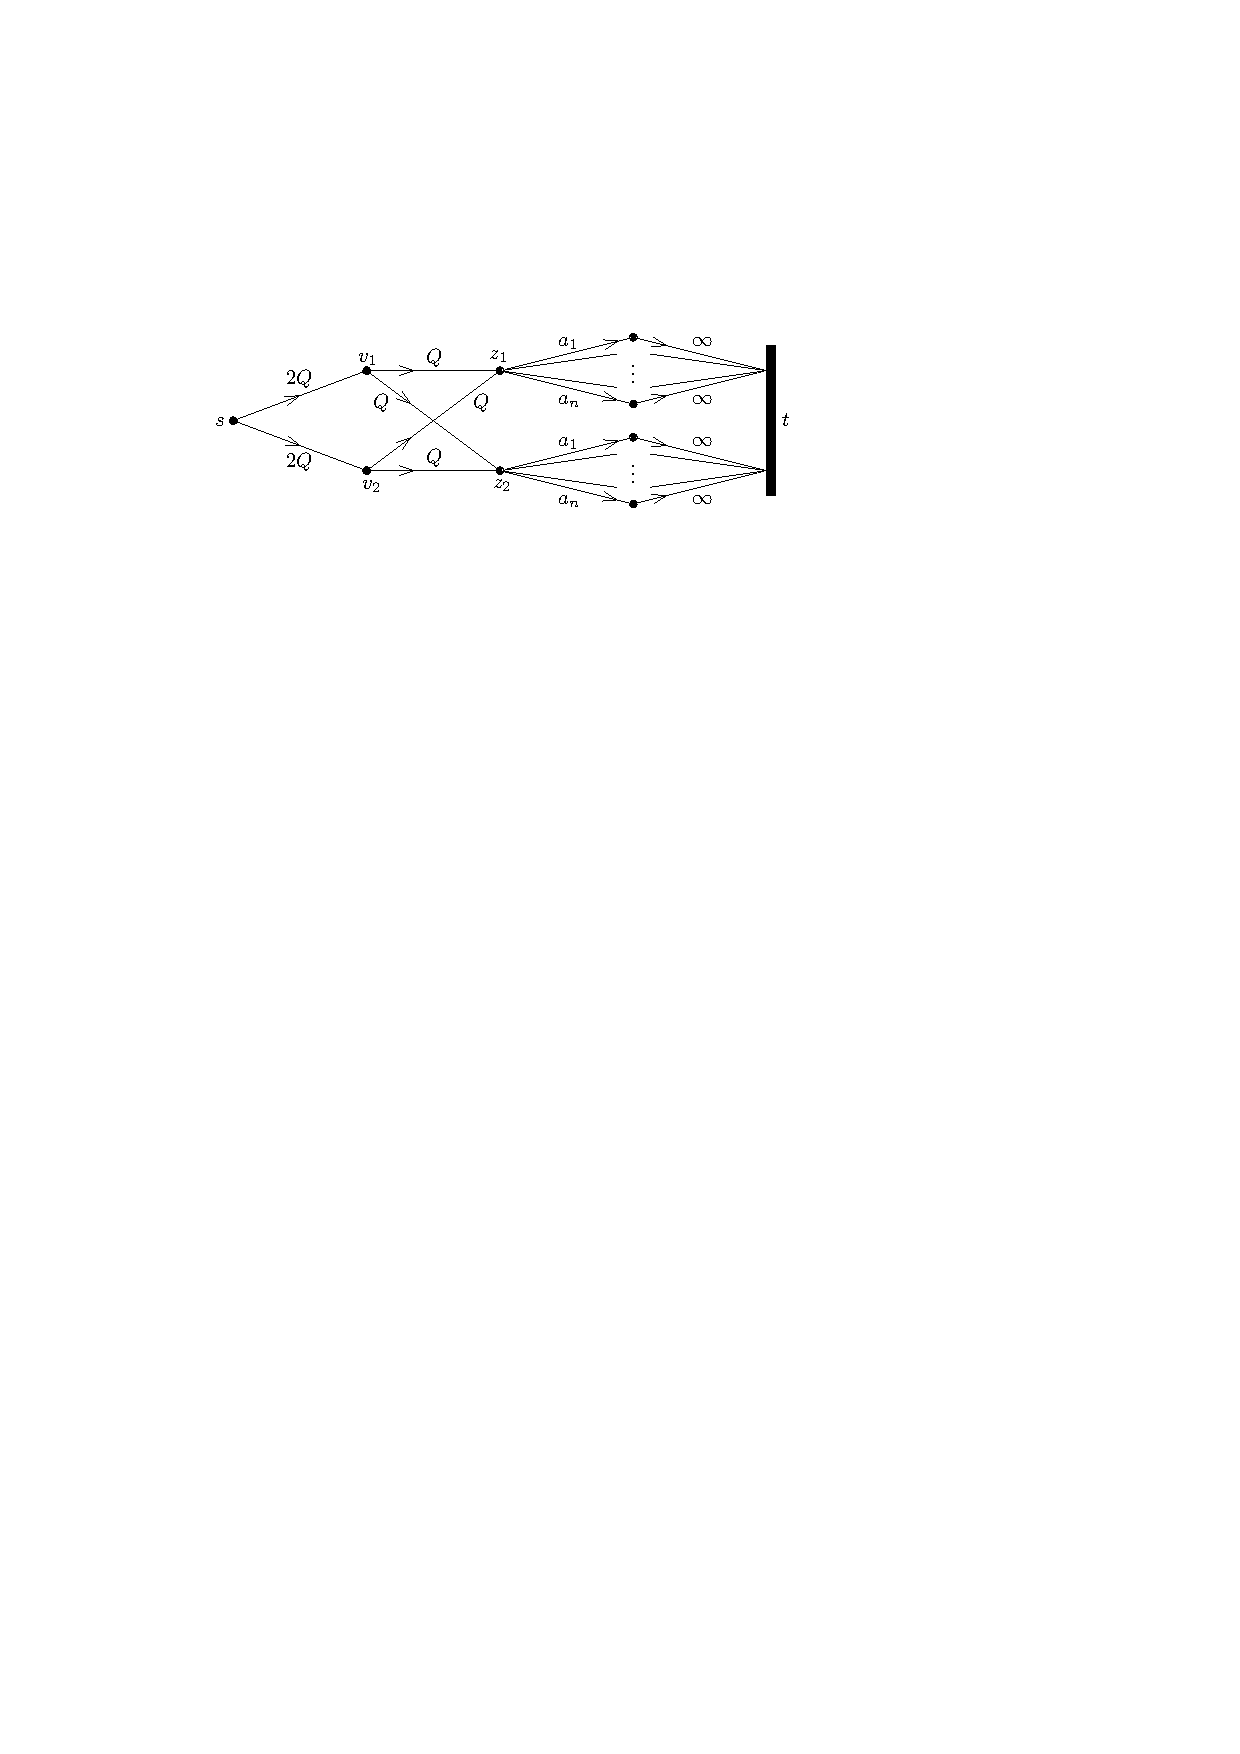
\includegraphics[scale=1]{img/st-act-np-hard}
\caption{Reduction \textsc{Partition} $\rightarrow$ \stact\ described in \cref{thm_stact_np_hard}.}
\label{fig_stact_np_hard}
\end{figure}

We wish to prove that \stact\ is NP-complete, even if the weights are restricted to $\set{1, 2}$. The idea is to introduce a gadget $G_k$, whose edges have weight restricted to $\set{1,2}$, such that $G_k$ behaves almost the same way as a single edge of weight $2k - 1$. The gadget is depicted in \cref{fig_gadget}. Formally, for $i \in [k]$, the edges $(s, v_i)$, $(z_i, t)$ have weight 2 each, and the edges $(v_i, z_i)$, $(v_i, z_{i+1})$ have weight 1 each (we let $z_{k+1} := z_1$).

\begin{lemma}
\label{lemma_gadget}
Let $G_k$ be the digraph depicted in \cref{fig_gadget}. Let $\sigma$ be a schedule for $G_k$ and let $C(\sigma)$ be like in \cref{sec_notation}. Then we have that \begin{enumerate}[(i)]
\item $|C(\sigma)| \leq 2k -1$,
\item $|C(\sigma)| = 2k -1$ can be achieved for some $\sigma$, and
\item If $|C(\sigma)| = 2k -1$, then $C(\sigma)$ is a set of $2k-1$ consecutive integers.
\label{lemma_gadget_case_3}
\end{enumerate}
\end{lemma}
\begin{proof}
For claim (i), observe that if we would use all edges to their full capacity, we would get a value of $2k$. However, due to the properties of nonpreemptive schedling, this is impossible to realize. Claim (ii) is easy to see. For claim (iii), assume the contrary, i.e.\ $|C(\sigma)| = 2k -1$ and $C(\sigma) = I_1 \cup \dots \cup I_m$ where $m \geq 2$ and $I_j = \fromto{a_j}{b_j}$ and $a_{j+1} \geq b_j + 2$ for all $j < m$. Then at least one of the intervals, say $I_1$, has an odd cardinality. Because  all edges have weight at most 2, we have that the set of edges contributing to $I_1$ (i.e.\ the set $E_1 := \set{e \in E(G_k) : \sigma(e) < b_1}$) is disjoint from the set of edges contributing to $I_2$ (i.e.\ the set $E_2 := \set{e \in E(G_k) : \sigma(e) + w(e) > a_2 - 1}$). Consider the cuts $\delta(s)$ and $\delta(t)$, both of which have capacity $2k$. Because $|I_1|$ is odd, but the edges in $\delta(s)$ and $\delta(t)$ have weight 2, at least one unit of capacity from both $\delta(s)$ and $\delta(t)$ is wasted in $E_1$. Now, applying a similar argument like in claim (i) to $E_2$ and $I_2$ yields $|C(\sigma)| < 2k - 1$, a contradiction. (If the interval of odd cardinality is not $I_1$, an analogous argument holds.)
%and $C(\sigma)$ is not an interval. Let $t_0 := \min C(\sigma)$. Because at most one unit of time from each of the cuts $\delta(s)$ or $\delta(t)$ is \enquote{wasted}, but at time $t_0 + 1$ a unit either in $\delta(s)$ or $\delta(t)$ is wasted, we have $t_0 + 1 \not\in C(\sigma)$. But then at time $t_0 + 2$ the situation looks isomorphic to \cref{fig_gadget} (b) and together with $v_1w_2$ and $v_kw_1$ we have already wasted 4 units of time. However, if we want to achieve a value of $2k - 1$ we can at most waste 3 units.
\end{proof}
\begin{figure}[htpb]
\centering
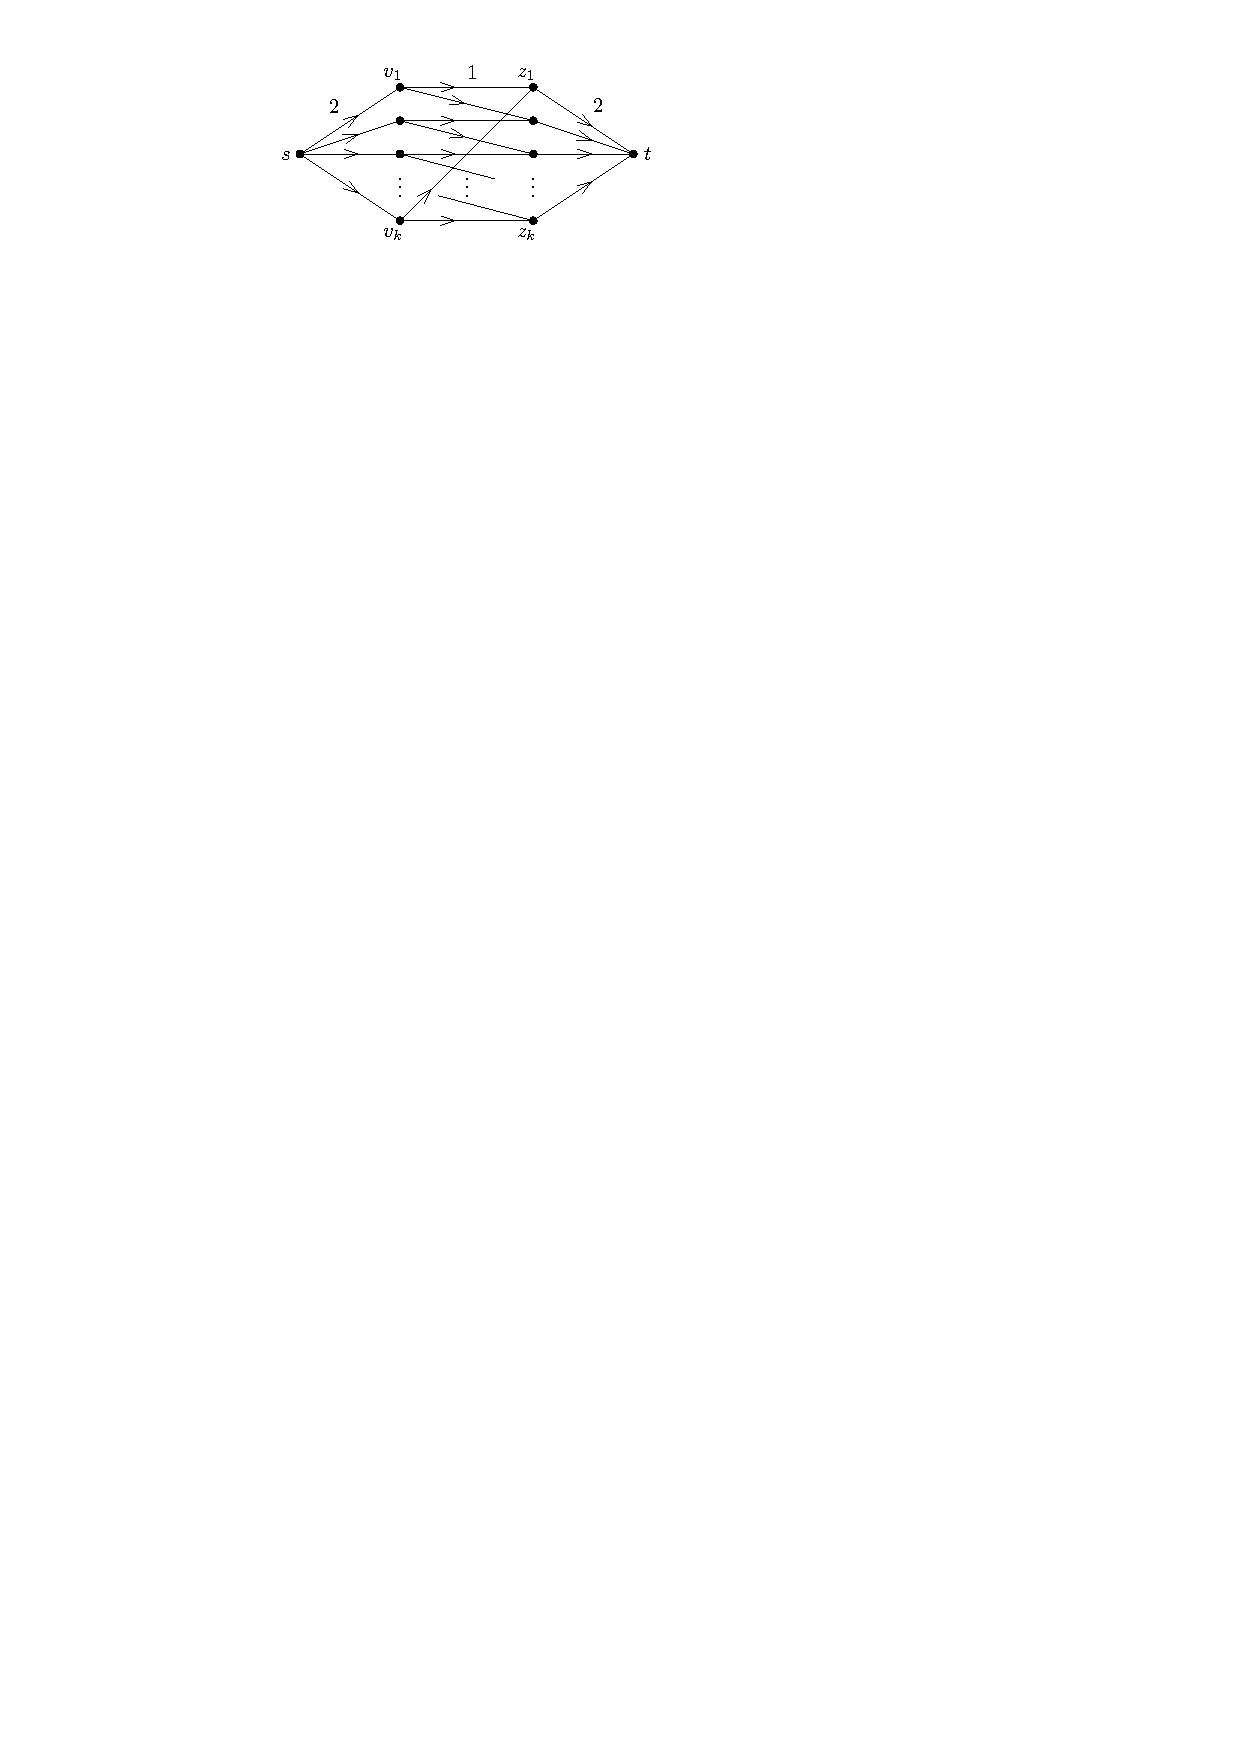
\includegraphics[scale=1]{img/gadget-new}
\caption{Gadget graph $G_k$.}
\label{fig_gadget}
\end{figure}

Having proven \cref{lemma_gadget}, it is natural to try the same hardness proof as \cref{thm_stact_np_hard}, and substitute an edge of weight $2k-1$ with the gadget $G_k$. This does not quite work, as the weights in this reduction are not polynomially bounded, hence the resulting graph is too large. However, if one considers instead a very similar reduction from \textsc{3-Partition}, one can prove:

\begin{restatable}{theorem}{stactonetwo}
\label{thm:stact_weights_one_two}
The problem \stact\ is NP-complete, even if $w(e) \in \set{1, 2}$ for all edges.
\end{restatable}

The resulting graphs do not have constant treewidth in this case. The full proof can be found in \cref{appendix:proof_stact_one_two}. 

\section{Relation between Problem and Relaxation}
\label{sec:ratio_relaxation}
The relaxation of problem \stact\ is Menger's problem. Given a fixed instance of $\stact$, how big can the ratio between its optimal solution $\optDirStAct$, and the optimal solution of the relaxation be? In this section, we show that it can be arbitrarily big. We describe an instance on $2n+2$ vertices, such that the solution to Menger's problem is $n^2$, but  $\optDirStAct = \theta(n^{1.5})$. In order to prove an upper bound for $\optDirStAct$, we make use of some tools from extremal graph theory. Namely, for vertices $x$ and $y$ in an undirected graph $H = (V, E)$, let $d(x, y) := \min\set{ |E(P)| : P \text{ is a $x$-$y$-path}}$ and $\radius(H) := \min_{x \in V} \max_{y \in V} d(x, y)$. Erd\H{o}s, Pach, Pollack and Tuza proved in 1987 \cite{erdHos1989radius}:
\begin{theorem}
\label{thm_mindegree_diameter_erdos}
Let $H$ be a connected, triangle-free, undirected graph with $N$ vertices, and with minimum degree $\delta \geq 2$. Then
\[\radius(H) \leq \frac{N-2}{\delta} + 12.\] 
\end{theorem}

\begin{theorem}
\label{thm_relaxation_ratio_unbounded}
In the instance $I = (G, w)$ depicted in \cref{fig_relaxation_ratio_unbounded} we have that the solution to Menger's problem is $n^2$, but for problem \stact\ one has
\[ \lfloor n^{0.5} \rfloor^3 \leq \optDirStAct(I)\leq  16 n^{1.5}\].
\end{theorem}
\begin{figure}[htpb]
\centering
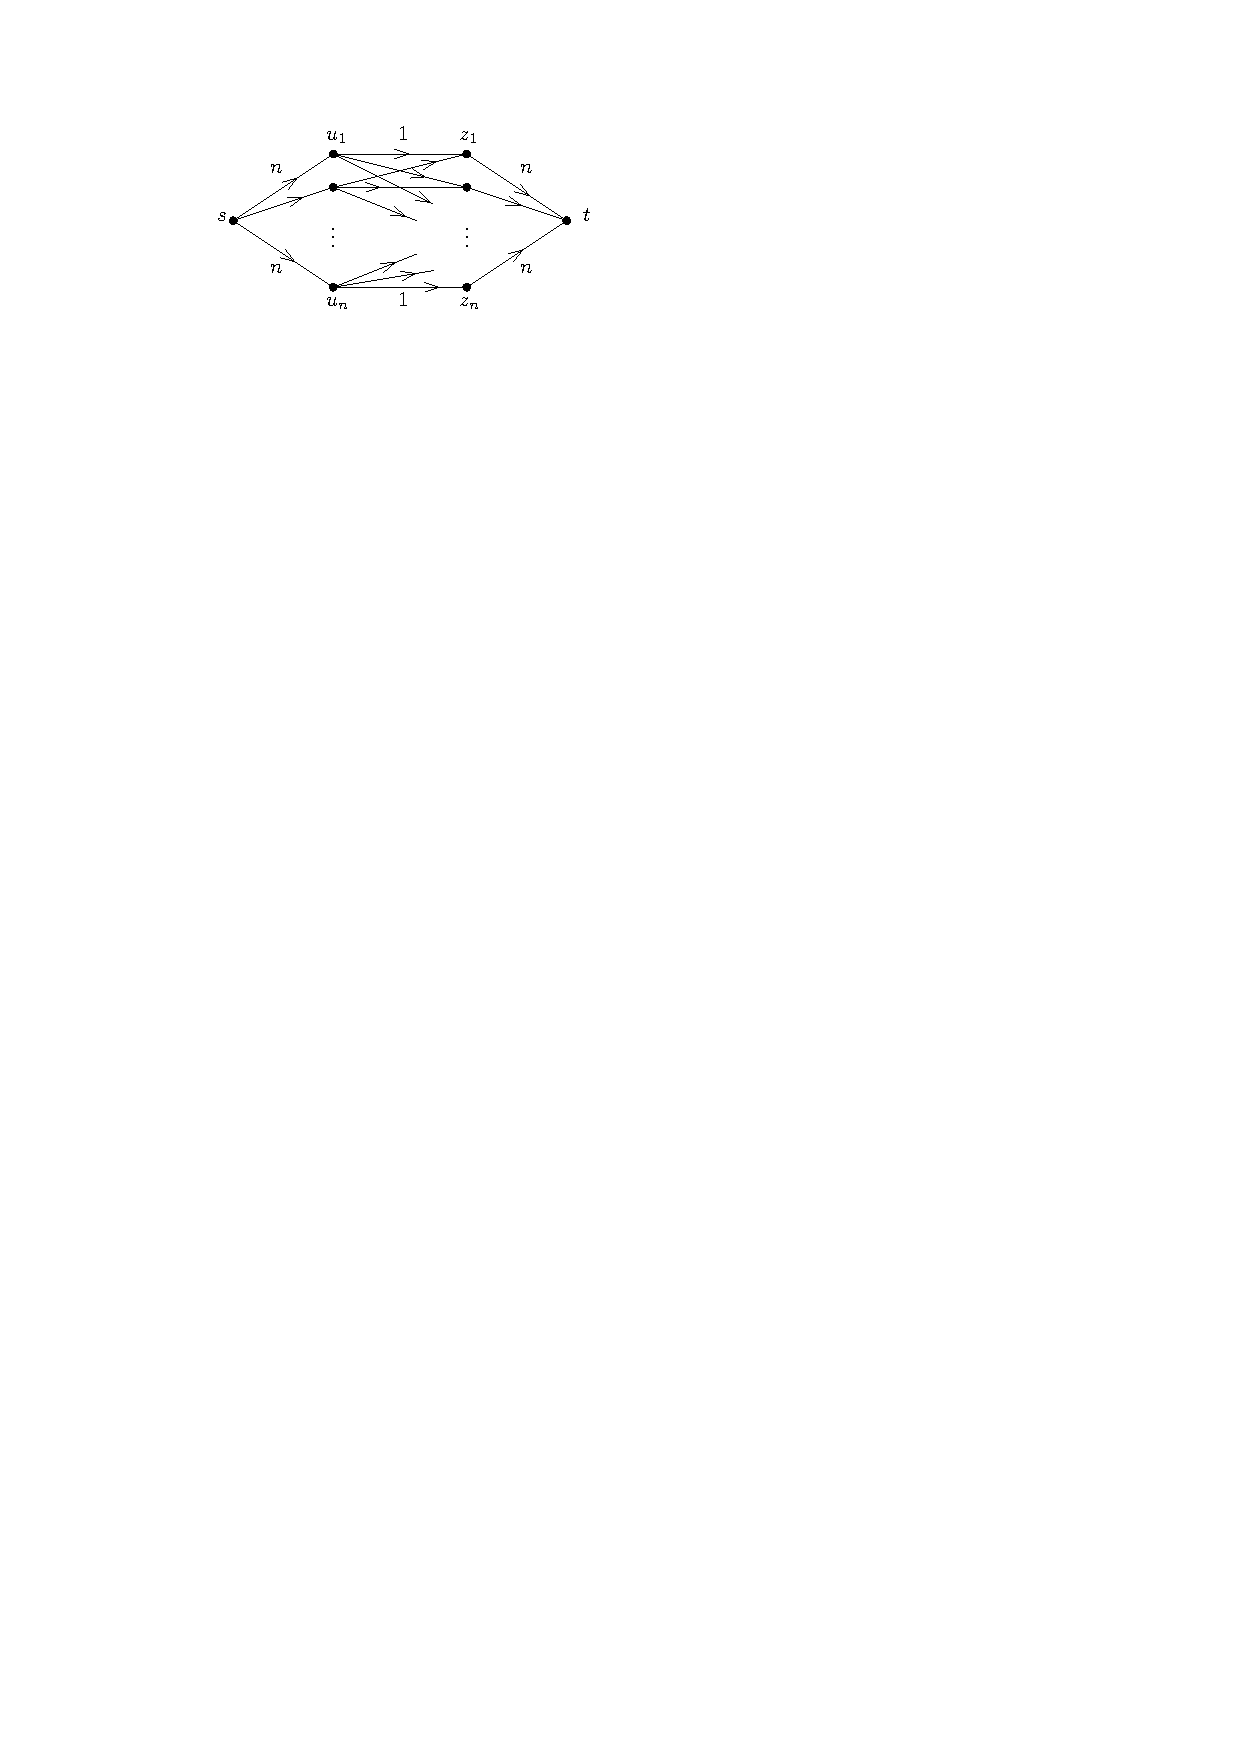
\includegraphics[scale=1]{img/relaxation-ratio-unbounded}
\caption{Graph used in the proof of \cref{thm_relaxation_ratio_unbounded}}
\label{fig_relaxation_ratio_unbounded}
\end{figure}
\begin{proof}
Let $G$ be the digraph sketched in \cref{fig_relaxation_ratio_unbounded}. Formally,  let $U := \fromto{u_1}{u_n}$ and $Z := \fromto{z_1}{z_n}$. For each $i$, there is an edge $(s,v_i)$ and  an edge $(z_i, t)$ with weight $n$ and for all $i, j$ there is an edge $(u_i, z_j)$ with weight 1. It is easy to see, that the optimal solution for the Menger problem for this instance is exactly $n^2$.
 First, we describe a schedule of value $\lfloor \sqrt{n} \rfloor^3$: Let $k := \lfloor \sqrt{n} \rfloor$ and consider for $i \in \fromto{1}{k}$ the sets $U_i := \fromto{u_{(i-1)k+1}}{u_{ik}}$ and $Z_i := \fromto{z_{(i-1)k+1}}{z_{ik}}$. Then consider the schedule consisting out of $k$ phases, where in the $i$-th phase, we activate all edges between $s$ and $U_i$ and all edges between $Z_i$ and $t$ at the beginning of the phase, and all $k^2$ edges between $U_i$ and $Z_i$ in order during the phase. It is easy to see that this describes a valid schedule of value $k^3$.
 
We now prove that $\optDirStAct(I) \leq 16n^{1.5}$. So assume there exists a schedule $\sigma$ of value greater than $T := 16n^{1.5}$. Then, for each $k \in \fromto{1}{T}$, there is at least one path $P_{k}$ from $s$ to $t$ in $G^\sigma_{k}$. Let $(u_{i(k)}, z_{j(k)})$ be the unique edge on $P_k$ which connects $U$ and $Z$ and $e_{k} := \{u_{i(k)}, z_{j(k)}\}$ be the corresponding undirected edge. For $k \neq k'$ we have $e_{k} \neq e_{k'}$. Consider the undirected graph $H'$ on vertex set $U \cup Z$ and edge set $\fromto{e_1}{e_T}$. 
%Then $H'$ has average degree $2E(H') / V(H') \geq T/n$. 
We claim there is a subgraph $H$ of $H'$ which is connected and has minimum degree at least $T/(2n)$. Indeed, note that $H'$ has the property that $|E(H')| \geq T/(2n)|V(H')|$ and deleting vertices of degree less than $T/(2n)$ does not change this property. Hence we can delete those vertices until we arrive at a graph with minimum degree at least $T/(2n)$ and $H$ can be chosen as any connected component of this graph. Now, \cref{thm_mindegree_diameter_erdos} applied to $H$ yields
\begin{equation}
\radius(H) \leq 2n\frac{|V(H)| - 2}{T} + 12  \leq \frac 1{8}|V(H)|n^{-0.5}+12. \label{eq_radius}
\end{equation}
For $u_i \in U$, define $\sigma(u_i) := \sigma((s,u_i))$ and for $z_j \in W$, define $\sigma(z_j) := \sigma((z_j,t))$. Now, a crucial observation is that by the definition of $e_k$, for each $k$ we have that both $(s,u_{i(k)}), (z_{j(k)}, t) \in E(G_k^\sigma)$, and therefore $|\sigma(u_{i(k)}) - \sigma(z_{j(k)})| \leq n - 1$. Define 
\[ L := \max_{v \in V(H)}\set{ \sigma(v) + n } - \min_{u \in V(H)} \set{\sigma(v)}, \]
 i.e.\ $L$ describes the theoretically maximal amount of time, such that $P_k$ could contain some vertex of $V(H)$. Let $R := 1/8|V(H)|n^{-0.5} +12$. By \cref{eq_radius} and the previous observation, and by $|V(H)| \geq \delta(H) \geq 8n^{0.5}$, we have 
\begin{align*}
L &\leq 2R(n-1) + n < (2R + 1)n = 1/4|V(H)|n^{0.5} + 25n\\ 
&\leq 1/4|V(H)|n^{0.5} + 25/8|V(H)|n^{0.5} < 4|V(H)|n^{0.5}.
\end{align*}
But on the other hand, $H$ has only edges of the form $e_k$, and by definition of $L$ and $e_k$ we must have $L \geq |E(H)| \geq |V(H)|\delta(H)/2 \geq 4|V(H)|n^{0.5}$. This is a contradiction.
\end{proof} 

%(Note: A more careful calculation in the previous proof yields $\optDirStAct(I) \leq 6\sqrt{6}n^{1.5}$.)

%\begin{corollary}
%There is a directed graph on $2n+2$ vertices such that $\optDirSTP = n^2$, but $\optDirAct = \theta(n^{1.5})$.
%\end{corollary}
%\begin{proof}
%Let $G$ be the same directed graph like in \cref{thm_relaxation_ratio_unbounded} with additional edges $(t, u_i)$ and $(t, w_i)$ for all $i$, each having weight $\infty$. Then finding a spanning branching in $G$ is equivalent to finding an $s$-$t$-path in the original graph, hence the claim follows by \cref{thm_relaxation_ratio_unbounded}.
%\end{proof}

Unfortunately, the idea for the proof of \cref{thm_relaxation_ratio_unbounded} can not be adapted to the case of undirected graph. Let (for even $n$) $G$ be the graph depicted in \cref{fig_relaxation_ratio_unbounded}, but without edge directions, i.e.\ we have $U = \fromto{u_1}{u_n}$, $Z := \fromto{z_1}{z_n}$ and undirected edges $\set{s, u_i}$ and $\set{z_i,t}$ of weight $n$ and undirected edges $\set{u_i, z_j}$ of weight 1 for all $i, j$. Then let $H := G[\fromto{u_{n/2+1}}{u_n} \cup \fromto{z_{n/2+1}}{z_n}]$ and fix some edge-coloring of $H$ with $n/2$ colors. Then consider the schedule consisting out of $n/2$ phases, where in the $i$-th phase we activate $\set{s,u_i}$, $\set{z_i,t}$, all edges of color $i$, and all edges $\set{u_i,z_j}$ and $\set{u_j,z_i}$ for $j \in \fromto{n/2+1}{n}$. This schedule has value $n^2/4$. So we can achieve a ratio of at least 1/4 of the solution to the Menger problem in this particular graph.

\appendix

\section{Proof of \cref{thm:stact_weights_one_two}}
\label{appendix:proof_stact_one_two}

The proof is in two steps. First, we prove a weaker result:

\begin{lemma}
\label{lemma_st_act_strongly_np_hard}
The problem \stact\ is strongly NP-complete. 
\end{lemma}
\begin{proof}
Let $A = \fromto{a_1}{a_{3n}}$ be an instance of \textsc{3-Partition} and $Q := 1/n \sum A$. Consider the digraph sketched in \cref{fig_stact_strongly_np_hard}. Here, there is an edge of weight $nQ$ between $s$ and $v_i$ for all $i$, there is a complete bipartite digraph between $\fromto{v_1}{v_n}$ and $\fromto{z_1}{z_n}$ with every edge having weight $Q$. Furthermore, the symbol $A$ in the figure represents $3n$ parallel edges with weights $a_1, \ldots, a_{3n}$ (compare \cref{fig_stact_np_hard}). We claim there is a schedule of value $n^2Q$, if and only if $A$ can be 3-partitioned. If $\sigma$ is such a schedule, we can assume by ($n$-fold) symmetry, that $\sigma((s, v_i)) = (i - 1)nQ$ for all $i \in [n]$. Let for $i \in [n]$, $P_i := [(i-1)nQ, inQ]$ denote the $i$-th phase of $\sigma$. During $P_i$, the edges $\fromto{(v_i,z_1)}{(v_i,z_n)}$ get activated in some order, let $(v_i,z_{f(i)})$ be the last edge in this order. Call a vertex $z_j$ exceptional, if $z_j = z_{f(i)}$ for some $i \in [n-1]$. At least one vertex $z'$ is not exceptional. Because $z'$ is not exceptional, the set of timesteps, where $z'$ is part of an $s$-$t$-path of active edges, consists out of $n$ distinct blocks of length $Q$ each, such that between two blocks there is a gap. Therefore the scheduling of the edges between $z'$ and $t$ implies a 3-partition of $A$. The other direction of the claim is easy to see.
\end{proof}
\begin{figure}[htpb]
\centering
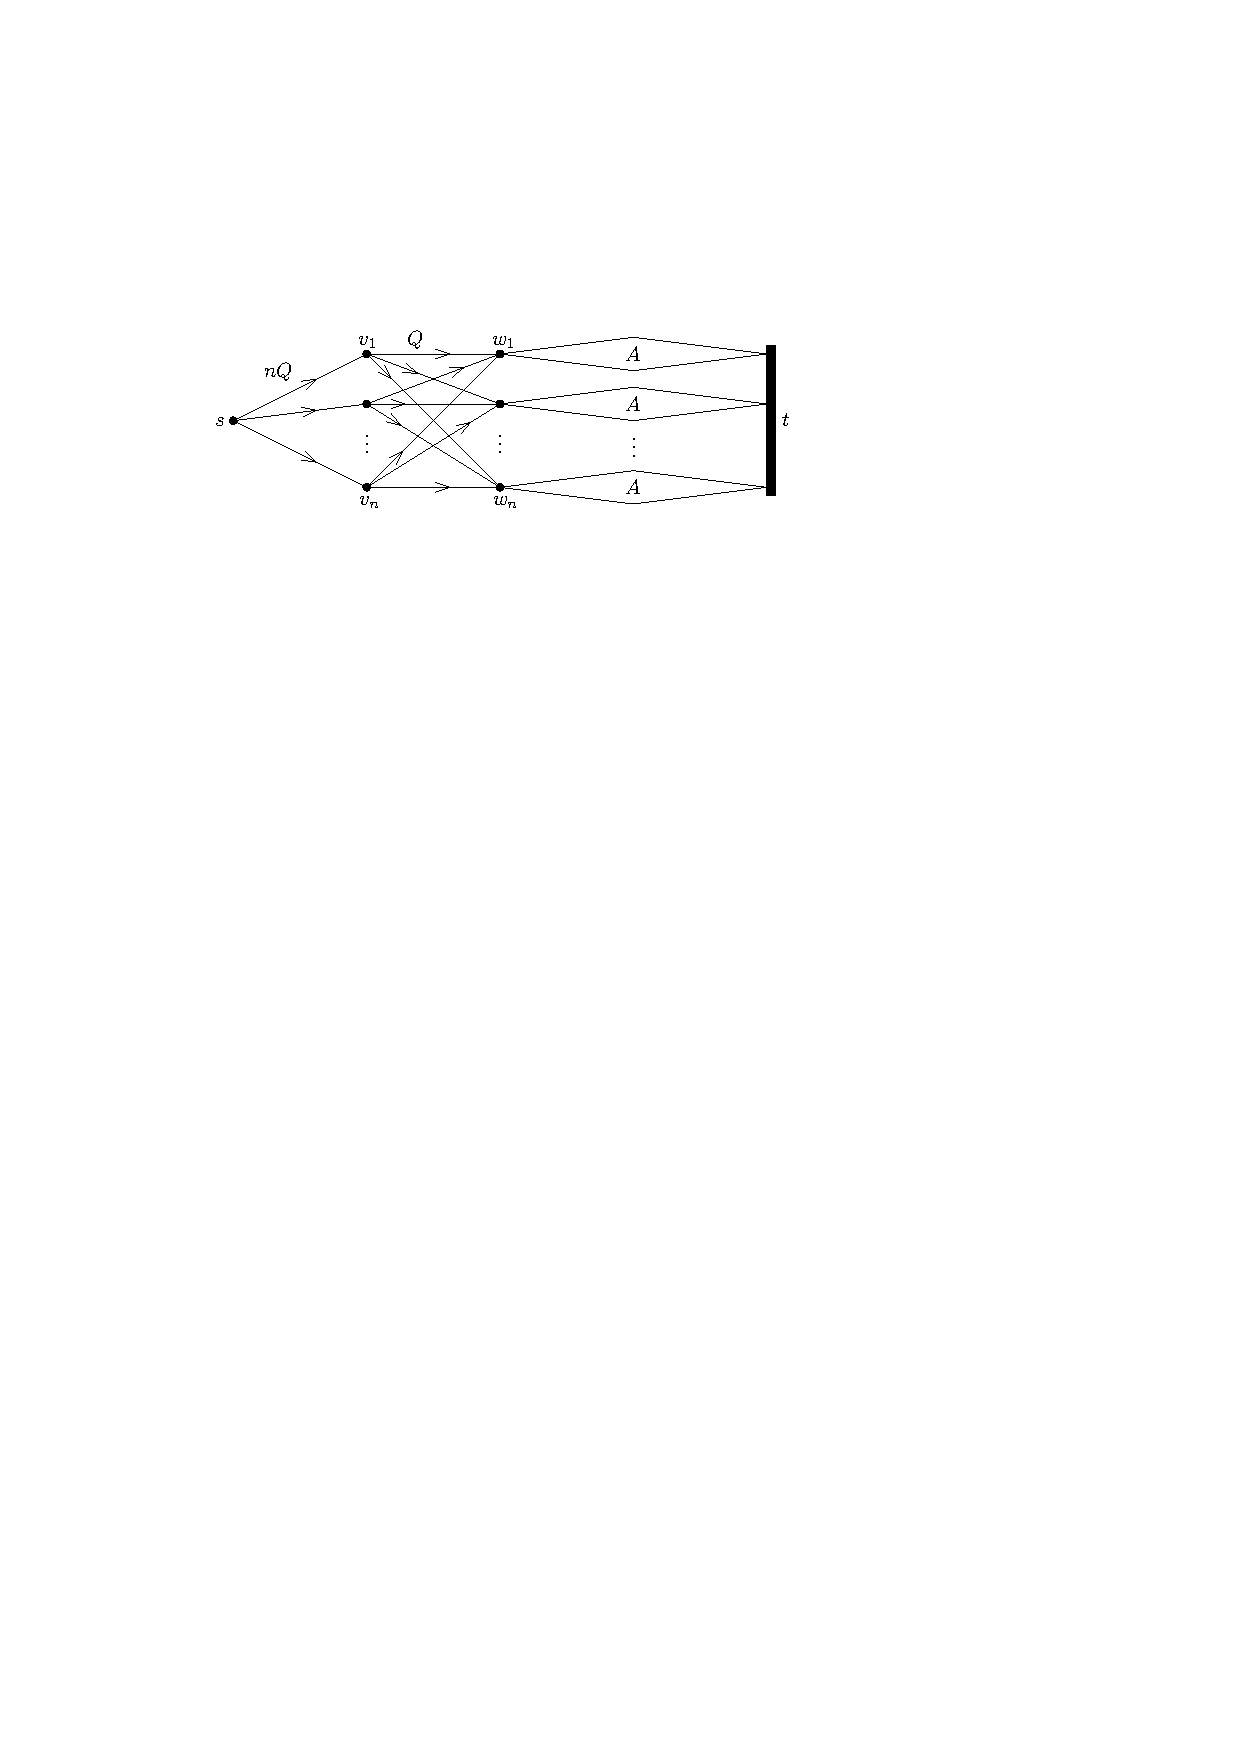
\includegraphics[scale=1]{img/st-act-strongly-np-hard}
\caption{Reduction \textsc{3-Partition} $\rightarrow$ \stact\ described in \cref{lemma_st_act_strongly_np_hard}.}
\label{fig_stact_strongly_np_hard}
\end{figure}


\stactonetwo*
\begin{proof}
Reduction from \textsc{3-Partition}. Let $A = \fromto{a_1}{a_{3n}}$ be an instance of \textsc{3-Partition} and let $Q := 1/n \sum A$, such that $a_i \leq p(n)$ for a suitable polynomial $p$. We can assume that $n$ is odd (otherwise, let $a_{3n+1} = a_{3n + 2} := 1$ and $a_{3n + 3} :=  Q - 2$) and each $a_i$ is odd (otherwise, let $a_i' := 2a_i + 1$). Then $Q$ is also odd. Now, consider the same reduction as in \cref{lemma_st_act_strongly_np_hard}, where we substitute an edge of weight $2k - 1$ by the gadget $G_k$. If a schedule of value $n^2Q$ exists, we need to use each gadget to its full extent, and therefore \cref{lemma_gadget} (iii) is applicable. Making use of \cref{lemma_gadget}, the rest of the proof is analogous to \cref{lemma_st_act_strongly_np_hard}.
\end{proof}

\section{Proof sketch that integrality gap for tree packing is at most log(n)}
The proof is from Anders Martinsson who mentioned it to me in private conversation after hearing a talk about non-preemptive tree packing.

The following lemma uses random scheduling of the edges and implies that the integrality gap of non-preemptive tree packing is at most $O(\log n)$. It also implies a randomized $O(\log n)$-approximation algorithm.

\begin{lemma}
There is $c > 0$ such that the following holds: Let $(G, w)$ be an instance of the non-preemptive tree packing problem, and let $k$ be the weight of a minimum weight cut. If $T = ck\log n$ and every edge is scheduled uniformly at random in the interval $[0, T]$, then with probability at least 1/2 the graph is connected for at least $T/4$ time slots.
\end{lemma}
\begin{proof}
(ToDo: Need to specify what exactly is meant by scheduling an edge uniformly randomly in $[0,T]$. What we want is that for every time slot and edge $e$, the edge is active during this time slot with probability $w(e)/T$. Observe that choosing the start point randomly in $[0, T-w(e)]$ does not have this property. Choosing the starting point randomly in $[-w(e), T-w(e)]$ is probably a good way to go - guarantees at least $w(e)/(3T)$.)

We are going to use the fact that the number of different minimum weight cuts is at most $O(n^2)$. In fact, this  is a well-known fact which follows from Karger's contraction algorithm (we sketch the argument for convenience).
As the graph has a min-cut of size $k$, it follows that if we are in the $i$-th step of Karger's algorithm where $n' = n-i$ vertices remain, then every vertex has minimum (weighted) degree $k$. Therefore the probability of success is at least $1 - k/(kn'/2)$.

The probability that a fixed minimum weight cut survives the contraction procedure is therefore
\[\prod_{i=0}^{n-3} (1 - \frac{2}{n-i}) = {n \choose 2}^{-1}.
\]
For different minimum cuts these are disjoint events and therefore there are at most ${n \choose 2} = \Theta(n^2)$ different minimum weight cuts.

This argument can be extended: Let $\alpha \geq 1$ and let $C$ be a cut of weight $\alpha k$. The probability that $C$ survives the contraction algorithm can be shown to be at least $n^{-c_0\alpha}$ for some constant $c_0 > 0$. Therefore there are at most $n^{c_0\alpha}$ cuts of weight $k\alpha$. Details for the proof of this known for example be found in Shayan Oveis Gharan's lecture notes (section on Karger's algorithm).

In the following argument, consider a fixed time slot $i \in \fromto{1}{T}$. Given a fixed cut $C$ of weight $k\alpha$, 
we observe that $C$ disconnects the graph during time slot $i$ if and only if none of its edges are active at time slot $i$. An edge is active at time slot $i$ with probability at least $w(e)/(3T)$ and the edges are scheduled independent of each other.
 Therefore the probability that $C$ is disconnected at time slot $i$ is at most 
\[
\prod_{e \in C}(1-\frac{w(e)}{3T}) \leq \prod_{e \in C} e^{-w(e)/(3T)} = e^{-w(C)/(3T)} = e^{-\alpha/(3c \log n)}.
\]
There are at most $n^{c_0\alpha}$ cuts of weight $k\alpha$. It follows by union-bound that the probability that at least one cut of size $k\alpha$ disconnects the graph at time step $i$ is at most 
\[ n^{c_0\alpha} e^{-\alpha/(3c \log n)} = e^{-\alpha c_0/(3c)}.\]
Using again union-bound, we see that the probability that there exists some cut which is disconnected during time slot $i$ is at most
\[\int_{\alpha=1}^\infty e^{- c_0/(3c)\alpha} \, d\alpha =  \frac{3c}{c_0}e^{-c_0/(3c)}.\]
If the constant $c$ is small enough, we see that the right-hand side of this expression can be made to be smaller than 1/2. In this case, for every time slot we have that the probability that the graph during this time slot is connected is at least 1/2. Therefore the expected number of time slots where the graph is connected is at least $T/2$. By Markov's inequality, we finally get
\[P(\text{Connected for at least $T/4$ time slots}) \geq 1/2.\]   
\end{proof}

\section{Possible idea relaxation ratio undirected}

\comment{Maybe can be proven with following idea: Use the graph in \cref{fig_undirected_relaxation_ratio} with a similar argument to the previous proof and additionally Szemeredi's regularity lemma???}
\begin{figure}[htpb]
\centering
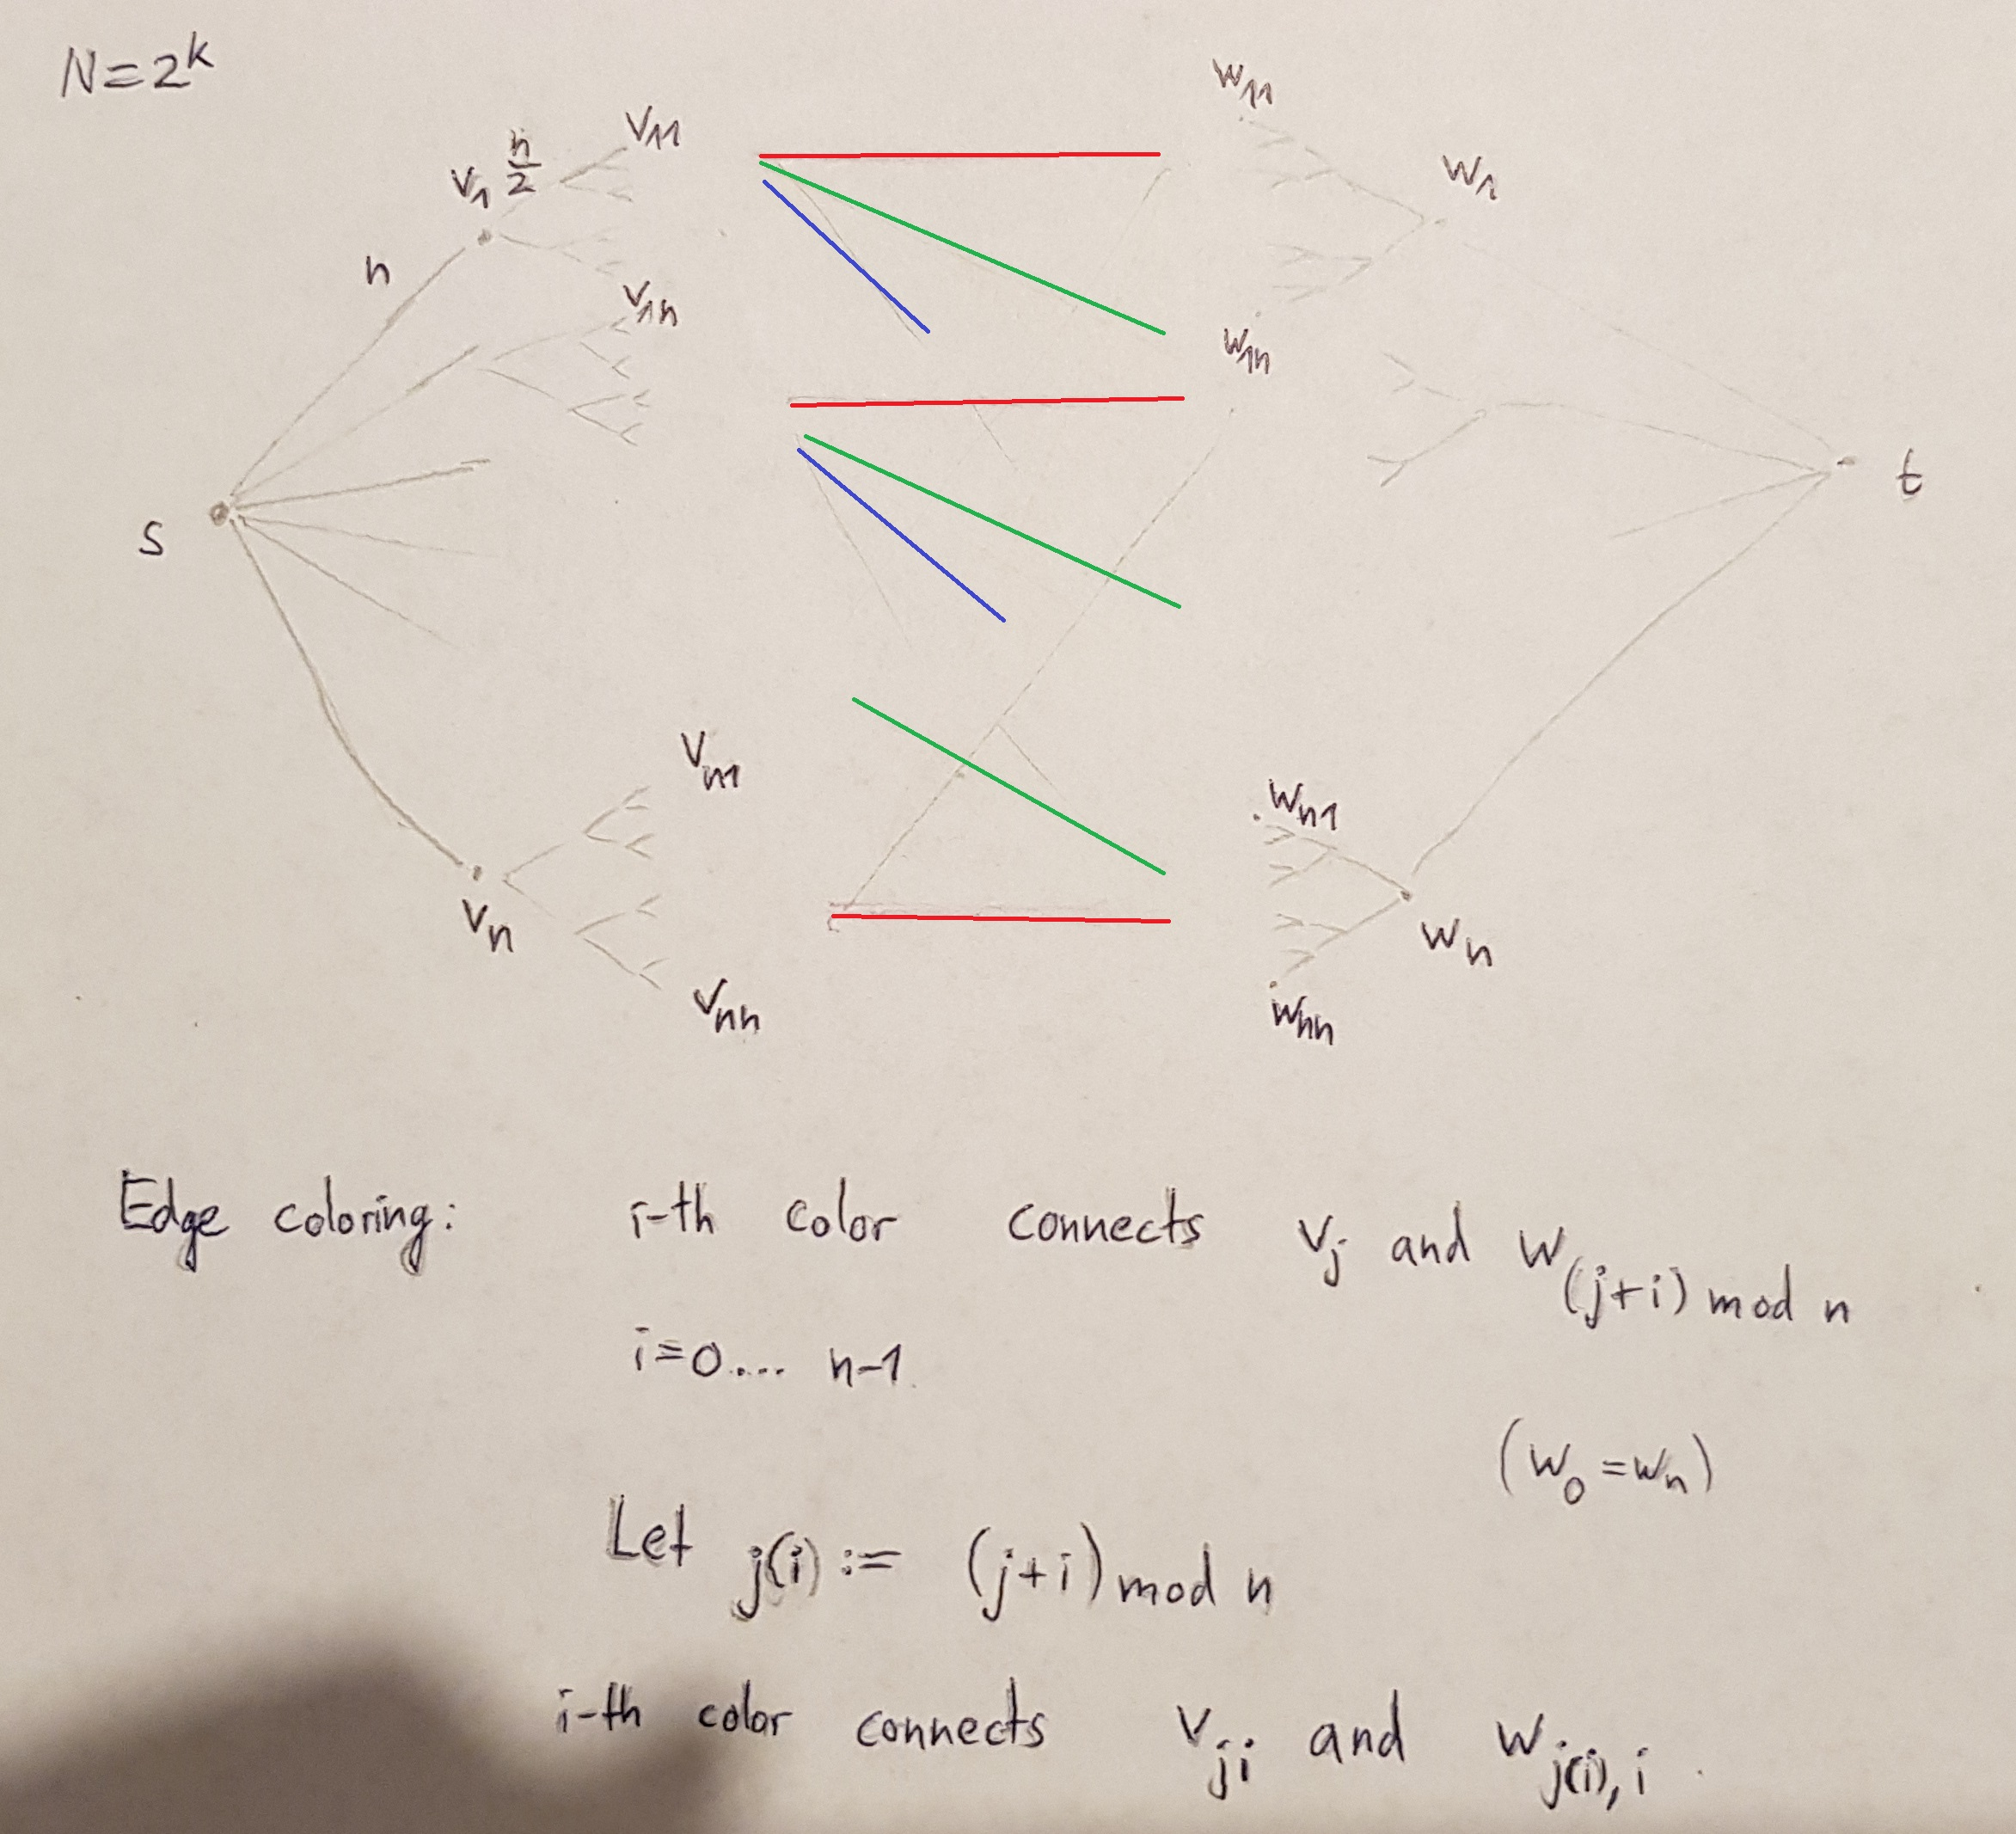
\includegraphics[width=\textwidth]{img/idea_undirected_approximation_ratio.jpg}
\caption{\comment{idea for proving an analogue of \cref{thm_relaxation_ratio_unbounded} for undirected graphs?}}
\label{fig_undirected_relaxation_ratio}
\end{figure}

\end{document}